\documentclass[30pt,twocolumn,letterpaper]{article}
\usepackage{cvpr}
\usepackage{times}
\usepackage{booktabs}
\usepackage{epsfig}
\usepackage{graphicx}
\usepackage{amsmath}
\usepackage{amssymb}
\cvprfinalcopy
\def\cvprPaperID{****}
\def\httilde{\mbox{\tt\raisebox{-.5ex}{\symbol{126}}}}
\usepackage{graphicx}
\usepackage{indentfirst}
\setlength{\parindent}{2em}
\usepackage{cite}
\usepackage[colorlinks,linkcolor=red,anchorcolor=blue,citecolor=green,backref=page]{hyperref}
\author{Qilei Zhang\\\\
Jun 10 2018}
\title{ImageNet Classification with Deep Convolutional Neural Networks}
\begin{document}
\maketitle
\begin{abstract}
  We trained a large, deep convolutional neural network to classify the 1.2 million high-resolution images in the ImageNet LSVRC-2010 contest into the 1000 different classes.
\end{abstract}
\section{Introduction}
Current approaches to object recognition make essential use of machine learning methods. To improve their performance, we can collect larger datasets, learn more powerful models, and use better techniques for preventing overfitting. Until recently, datasets of labeled images were relatively small �� on the order of tens of thousands of images\cite{Barat2016String}. \\
\begin{figure}[htbp]
\small
\centering
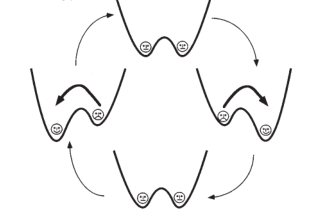
\includegraphics[width=20em]{000.png}
\caption{Transfer ratios on the Amazon benchmark. Both SDA-based systems outperforms the rest, and SDAsh (unsupervised training on all domains) is best.Reproduced from Glorot et al. (2011b).}
\label{fig:lable}
\end{figure}\\
\begin{equation}
\quad x'=f(x)+A_0cos(wt+o)+u(t)
\end{equation}
\section{The Dataset}
ImageNet is a dataset of over 15 million labeled high-resolution images belonging to roughly 22,000 categories. The images were collected from the web and labeled by human labelers using Amazon��s Mechanical Turk crowd-sourcing tool\cite{Mahendran2015Visualizing}. \\
\section{Reducing Overfitting}
Our neural network architecture has 60 million parameters. Although the 1000 classes of ILSVRC make each training example impose 10 bits of constraint on the mapping from image to label, this turns out to be insufficient to learn so many parameters without considerable overfitting. Below, we describe the two primary ways in which we combat overfitting\cite{Yi2010Effective}.
{\small
\bibliographystyle{ieee}
\bibliography{1}
}
\end{document}
